% Prof. Dr. Ausberto S. Castro Vera
% UENF - CCT - LCMAT - Curso de Ci\^{e}ncia da Computa\c{c}\~{a}o
% Campos, RJ,  2021
% Disciplina: Paradigmas de Linguagens de Programa\c{c}\~{a}o
% Aluno:



\chapter{ Aplica\c{c}\~{o}es da Linguagem Python}

A facilidade com que o Python pode ser escrito e interpretado, contribui para que a linguagem esteja presente em diversas áreas de atuação, que vai dês do desenvolvimento web, ate mesmo para a inteligência artificial, como o Machine Learning (aprendizado de maquina)


    \section{Opera\c{c}\~{o}es b\'{a}sicas}
        Python também é uma excelente linguagem par ser usada junto da matemática com sua sintaxe simplificada.
        Abaixo algumas demonstrações de operações básicas usando Python
        
\begin{lstlisting}
    #coding: utf-8


    # soma
    >>> 5+5
    # resultado = 10
    
    # subtração
    >>> 10-2
    # resultado = 8
    
    
    # multiplicação
    >>> 2*2
    # resultado = 4
    
    # divisão
    >>> 81/9
    # resultado = 9.0
    
    
    # exponenciação
    >>> 2**5
    # resultado = 32
    
    # extração da parte inteira da divisão
    >>> 10//9
    # resultado = 1

\end{lstlisting}

    \section{Programas gr\'{a}ficos}
        Por ser uma linguagem com uma comunidade muito grande, Python possui uma grande quantidade de bibliotecas e ferramentas, feitas pela comunidade e nativas da própria linguagem, que nos auxiliam a criar ate mesmo interfaces gráficas utilizando Python, uma dessas bibliotecas mais famosas é o Tkinter. 
        Um dos principais destaques do Tkinter para outras bibliotecas é que o Tkinter é nativo da linguagem Python, isso significa que não há necessidade de se instalar nenhum pacote a mais, apenas por ter o Python instalado, já se é possível usar o Tkinter.
        
        Abaixo um exemplo de código do Tkinter e a interface gerada por ele.

\begin{lstlisting}

from tkinter import *

class Application:
    def __init__(self, master=None):
        self.widget1 = Frame(master)
        self.widget1.pack()
        self.msg = Label(self.widget1, text="Primeiro widget")
        self.msg["font"] = ("Calibri", "9", "italic")
        self.msg.pack ()
        self.sair = Button(self.widget1)
        self.sair["text"] = "Clique aqui"
        self.sair["font"] = ("Calibri", "9")
        self.sair["width"] = 10
        self.sair.bind("<Button-1>", self.mudarTexto)
        self.sair.pack ()

    def mudarTexto(self, event):
        if self.msg["text"] == "Primeiro widget":
            self.msg["text"] = "O botão recebeu um clique"
        else:
            self.msg["text"] = "Primeiro widget"


root = Tk()
Application(root)
root.mainloop()

\end{lstlisting}

Abaixo na figura temos o seguinte resultado com esse código usando Tkinter.

 \begin{figure}[H]
    \begin{center}
        \caption{Resultado final da interface usando o Tkinter} \label{ling1}
        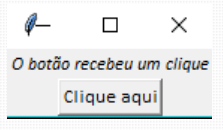
\includegraphics[width=12cm]{Pictures/python-UI.png} \\
    \end{center}
   \end{figure}
    
    \section{Programas com Objetos}
    Por ser uma linguagem orientada a objetos, Python trás uma forma muito simples todos os conceitos por baixo de Orientação a objetos, podemos ver no seguinte exemplo, a declaração de um objeto Pessoa, com seus atributos e métodos.

\begin{lstlisting}

class Pessoa:
    def __init__(self, nome, sexo, cpf, ativo):
        self.nome = nome
        self.sexo = sexo
        self.cpf = cpf
        self.__ativo = ativo
        
    def desativar(self):
        self.__ativo = False
        print("A pessoa foi desativada com sucesso")

if __name__ == "__main__":
    pessoa1 = Pessoa("João", "M", "123456", True)
    pessoa1.desativar()
    pessoa1.ativo = True
    print(pessoa1.ativo)
    
    
    # Resultado
    # A pessoa foi desativada com sucesso 
    # true

\end{lstlisting}

    \section{O algoritmo Quicksort - Implementa\c{c}\~{a}o}
    O QuickSort é um famoso algoritmo de ordenação, que se utiliza da estratégia de dividir para conquistar, assim conseguindo ordenar grande quantidade de números em um intervalo pequeno de tempo.
    Abaixo um exemplo da implementação de um QuickSort em Python e no final o seu resultado.
    
\begin{lstlisting}

def quickSort(alist):
   quickSortHelper(alist,0,len(alist)-1)

def quickSortHelper(alist,first,last):
   if first<last:

       splitpoint = partition(alist,first,last)

       quickSortHelper(alist,first,splitpoint-1)
       quickSortHelper(alist,splitpoint+1,last)


def partition(alist,first,last):
   pivotvalue = alist[first]

   leftmark = first+1
   rightmark = last

   done = False
   while not done:

       while leftmark <= rightmark and alist[leftmark] <= pivotvalue:
           leftmark = leftmark + 1

       while alist[rightmark] >= pivotvalue and rightmark >= leftmark:
           rightmark = rightmark -1

       if rightmark < leftmark:
           done = True
       else:
           temp = alist[leftmark]
           alist[leftmark] = alist[rightmark]
           alist[rightmark] = temp

   temp = alist[first]
   alist[first] = alist[rightmark]
   alist[rightmark] = temp


   return rightmark

alist = [54,26,93,17,77,31,44,55,20]
quickSort(alist)
print(alist)


# [17, 20, 26, 31, 44, 54, 55, 77, 93]

\end{lstlisting}

No final da ordenação obtemos o seguinte resultado acima 


    \section{Aplica\c{c}\~{o}es com Banco de Dados}
    Existem uma série de bibliotecas que podem ser utilizadas tanto para consumir o conteudo de um banco, quanto para criar um através do Python, nesse exemplo utilizaremos as seguintes bibliotecas, sqlalchemy, e pandas, para inserirmos valores nas querys do banco.
    
    caso tenha alguma dúdiva você pode encontrar a documentação do SQLAlchemy no link abaixo: 
    
    https://docs.sqlalchemy.org/en/latest/core/engines.html
    
    
\begin{lstlisting}
import pandas as pd
import sqlalchemy

# Criando a Conexão
engine = sqlalchemy.create_engine('mysql+pymysql://url_banco')

# Lendo toda a tabela Employees e transformando em DataFrame.
df = pd.read_sql_table('employees',engine)

# Listando os dados e informações dos atributos.
df.head()

\end{lstlisting}

\begin{figure}[H]
    \begin{center}
        \caption{Dados ilustrativos do banco} \label{ling1}
        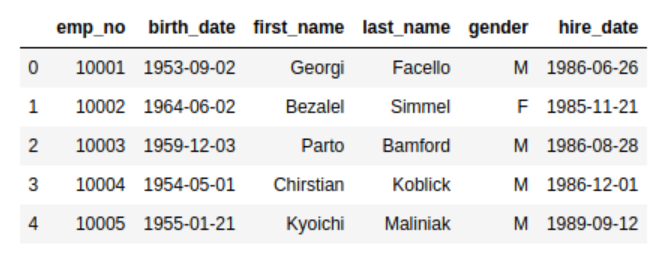
\includegraphics[width=12cm]{Pictures/python_database.png} \\
    \end{center}
\end{figure}

\begin{lstlisting}
# Criando um DataFrame a partir de uma query ao banco de dados.

df = pd.read_sql_query("select * from employees",engine)
\end{lstlisting}

O select * from employees retorna todos os dados da tabela employees.
